
% ほとんどの映像作品は状況を説明するオーバーレイキャプションを持つ
% 例えば球技の試合映像なら得点状況、旅行番組であれば地図、オペラならば歌詞などである
Almost every movie contents have overlaid captions or images that describe situations and provide supplementary information.
For example, a record of a ball game has a caption about the score, some TV programs about traveling would have overlaid maps, and a movie of a concert may have captions of words of songs.
% キャプション作成やタイミングを合わせて合成することは手間が掛かる
Making such captions and overlaying them in appropriate timings is a laborious part of a movie authoring process.
% AnnoToneにより状況を録画時に埋め込んでおくことで、多くの作業を自動化出来るだろう
In some cases, creating and overlaying captions would be able to be automated by embedding contextual information into videos and utilizing them by AnnoTone.

\begin{figure}[htbp]
 \begin{center}
  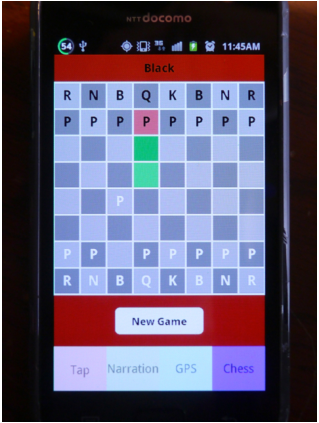
\includegraphics[height=60mm]{application_chess_app.pdf}
  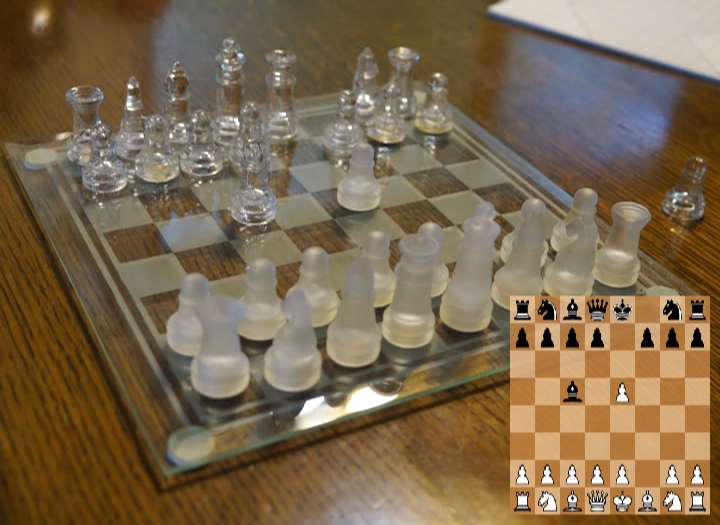
\includegraphics[height=60mm]{application_chess_movie.png}
 \end{center}
 \caption{Left: The user interface for annotating chess notes. Right: Movie overlaid with a chessboard by the system.}
 \label{fig:appl_chss}
\end{figure}

% 我々はチェスの記録映像を対象に、自動的に盤面状況を画面にオーバーレイするシステムを作成した。
As an illustration, we developed a system for chess movies that automatically overlay a video with an animation of a chessboard reflecting game progress using chess notes embedded in the video.
% アノテーションは、通常のプレイ時に棋譜を行うのと同様にプレイヤーまたはカメラマンが手動で行う
A camera operator or players operate a smartphone application to embed the chess notes in a video, like recording notes in ordinary games.
The application provides a video game-like simple user interface (shown in Figure \ref{fig:appl_chss} left) presenting a chessboard to easily record a game.
Each chess note is generated as a record of standard Forsyth-Edwards Notation (FEN) therefore the notes embedded in a video represents all information of a game.
% ソフトウェアが棋譜が埋め込まれた動画を解析し、各時点での盤面の状況を画面右下にオーバーレイする
The system analyzes a video annotated with chess notes to calculate the states of chessboard at each timestamps and generate a series of overlay images as shown in Figure \ref{fig:appl_chss} right.
